\documentclass[aspectratio=169,11pt]{beamer}

% Follow the supplied presentation reference: Madrid title treatment,
% conventional Beamer spacing, and a date / title / page footer.
\usetheme{Madrid}
\usecolortheme{default}
\usepackage{fontspec}
\setsansfont{Arial}
\setmainfont{Arial}
\usepackage{amsmath,amssymb}
\usepackage{graphicx}

\definecolor{MECBlue}{HTML}{3733B8}
\definecolor{Ink}{HTML}{203540}
\definecolor{Muted}{HTML}{536A78}
\definecolor{SignalOrange}{HTML}{BD5720}

\setbeamercolor{structure}{fg=MECBlue}
\setbeamercolor{frametitle}{fg=white,bg=MECBlue}
\setbeamercolor{title}{fg=white,bg=MECBlue}
\setbeamercolor{author in head/foot}{fg=white,bg=MECBlue}
\setbeamercolor{date in head/foot}{fg=white,bg=MECBlue}
\setbeamercolor{normal text}{fg=Ink,bg=white}
\setbeamercolor{block title}{fg=white,bg=MECBlue}
\setbeamercolor{block body}{fg=Ink,bg=blue!5}
\setbeamercolor{block title alerted}{fg=white,bg=SignalOrange}
\setbeamercolor{block body alerted}{fg=Ink,bg=orange!8}
\setbeamerfont{frametitle}{size=\large,series=\bfseries}
\setbeamerfont{title}{size=\LARGE,series=\bfseries}
\setbeamertemplate{navigation symbols}{}
\setbeamertemplate{blocks}[rounded][shadow=false]
\setbeamertemplate{title}[default][colsep=-4bp,rounded=true,shadow=false]

% Keep the familiar reference footer fields while allowing breathing room
% at both page edges. Fixed page-relative widths prevent right-edge clipping.
\setbeamertemplate{footline}{%
  \leavevmode
  \hbox{%
    \begin{beamercolorbox}[wd=\paperwidth,ht=2.25ex,dp=2ex]{author in head/foot}%
      \usebeamerfont{author in head/foot}%
      \hspace*{2ex}\insertshortdate
      \hfill
      \textbf{\insertshorttitle}
      \hfill
      \insertframenumber/\inserttotalframenumber
      \hspace*{2ex}%
    \end{beamercolorbox}%
  }%
  \vskip0pt
}

\title[Traffic Signal Timing]{Stochastic Traffic Signal Timing\\Optimization}
\subtitle{A queuing and Monte Carlo study}
\author[]{%
  \texorpdfstring{%
    \begin{tabular}{@{}l@{\hspace{1.2cm}}l@{}}
      \textbf{Dijith Dinesh} & \textbf{Athuljith S}\\[0.12cm]
      \textbf{Peter Joe Menachery} & \textbf{Pranav Manoj}
    \end{tabular}%
  }{Dijith Dinesh, Athuljith S, Peter Joe Menachery, Pranav Manoj}%
}
\institute{Department of Computer Engineering\\Government Model Engineering College, Thrikkakara}
\date[October 26, 2026]{October 26, 2026}

\begin{document}

% 1 — standard title page, following the supplied reference.
\begin{frame}
  \titlepage
\end{frame}

% 2 — research question and model boundary.
\begin{frame}{A precise, limited question}
  \begin{itemize}
    \setlength{\itemsep}{0.36cm}
    \item \textbf{Decision:} allocate 80 seconds of green time across the North, East, South, and West approaches.
    \item \textbf{Signal operation:} four protected phases in a 96-second cycle, including 16 seconds of clearance.
    \item \textbf{Scenario:} 12 movement queues, initially empty, with assumed Poisson arrivals over a 600-second period.
  \end{itemize}
  \vspace{0.28cm}
  \begin{block}{Objective}
    Minimize expected cumulative waiting, measured in vehicle-seconds. No field measurements are used in this primary experiment.
  \end{block}
\end{frame}

% 3 — the arrival process and queue-area measure.
\begin{frame}{From arrivals to waiting cost}
  \begin{columns}[T,onlytextwidth]
    \column{0.47\textwidth}
      \textbf{\large Poisson arrivals}

      \vspace{0.18cm}
      Uniform pseudorandom draws are transformed into exponential interarrival gaps:
      \[
        \Delta t=-\frac{\ln(1-U)}{\lambda}.
      \]
      A turning draw assigns each vehicle to a dedicated left, through, or right queue.
    \column{0.47\textwidth}
      \textbf{\large Queue-area objective}

      \vspace{0.18cm}
      \[
        D_T(\mathbf g)=\sum_{m=1}^{12}\int_0^T Q_m(t;\mathbf g)\,dt.
      \]
      This is cumulative waiting in vehicle-seconds, including partial waiting still in progress at the horizon.
  \end{columns}
  \vspace{0.24cm}
  \begin{block}{Matched comparison}
    Every candidate timing is scored against the same training arrivals to reduce noise in the search.
  \end{block}
\end{frame}

% 4 — the search and its evaluation procedure.
\begin{frame}{Search, then evaluate on fresh traffic}
  \begin{enumerate}
    \setlength{\itemsep}{0.28cm}
    \item Enumerate feasible green allocations on the selected timing grid.
    \item Score every candidate on shared training arrivals.
    \item Select the candidate with the lowest estimated mean waiting.
    \item Evaluate the selected plan on new, matched arrivals.
  \end{enumerate}
  \vspace{0.25cm}
  \begin{columns}[T,onlytextwidth]
    \column{0.47\textwidth}
      \textbf{Why simulation?}

      \smallskip
      Service stops at red and uses fixed headways. A continuously serving M/M/1 formula does not represent this signal operation exactly.
    \column{0.47\textwidth}
      \textbf{Reported measures}

      \smallskip
      Mean waiting, paired differences, queue profiles, residual backlog, and uncertainty intervals.
  \end{columns}
\end{frame}

% 5 — primary four-second-grid result.
\begin{frame}{The ten-minute reference result}
  \begin{columns}[T,onlytextwidth]
    \column{0.59\textwidth}
      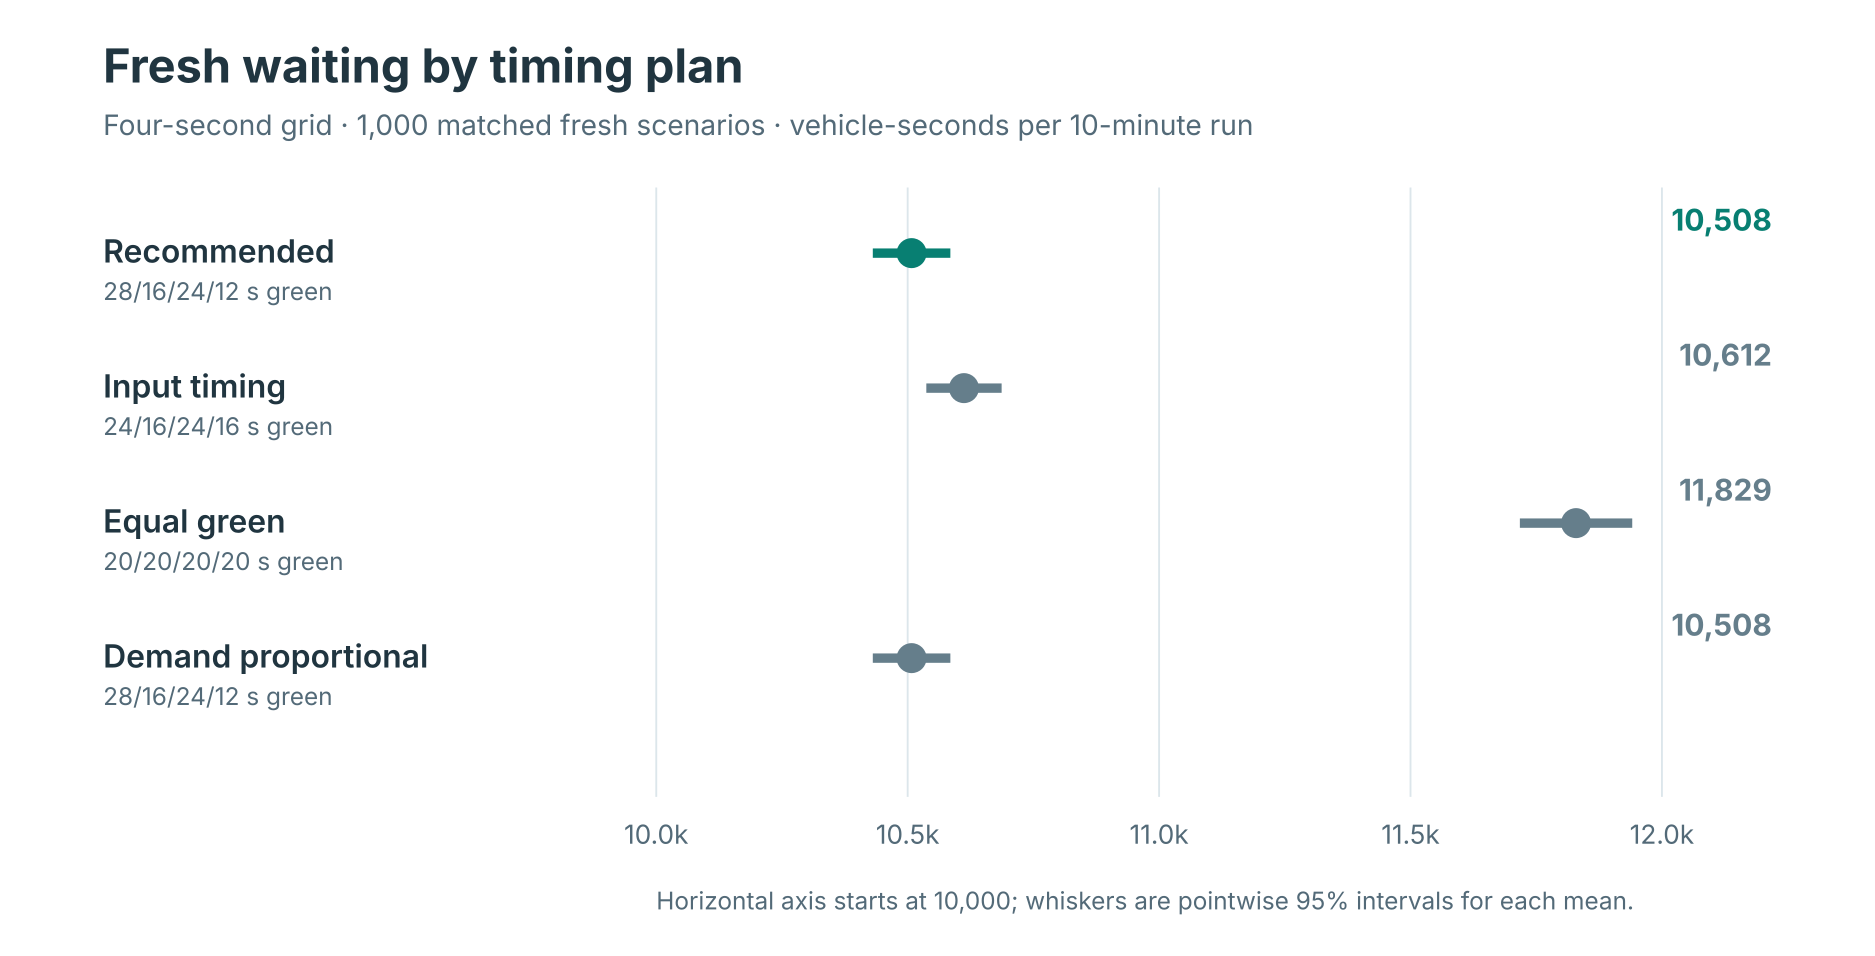
\includegraphics[width=\linewidth,height=0.58\textheight,keepaspectratio]{../assets/fig-timing.png}
    \column{0.37\textwidth}
      \textbf{\large Four-second-grid selection}
      \begin{itemize}
        \setlength{\itemsep}{0.12cm}
        \item Green (N/E/S/W): \textbf{28 / 16 / 24 / 12 s}
        \item Fresh mean: \textbf{10,507.8 vehicle-seconds/run}
        \item Saving vs entered timing: \textbf{104.2 vehicle-seconds/run}
        \item 1,000 fresh runs; paired 95\% interval: \textbf{69.6--138.8}
      \end{itemize}
  \end{columns}
  \vspace{0.12cm}
  \small\color{Muted}The selected plan equals the demand-proportional baseline; the mean reduction is modest.
\end{frame}

% 6 — one-second-grid selection and fresh evaluation.
\begin{frame}{Fine-grid timing result}
  \begin{columns}[T,onlytextwidth]
    \column{0.55\textwidth}
      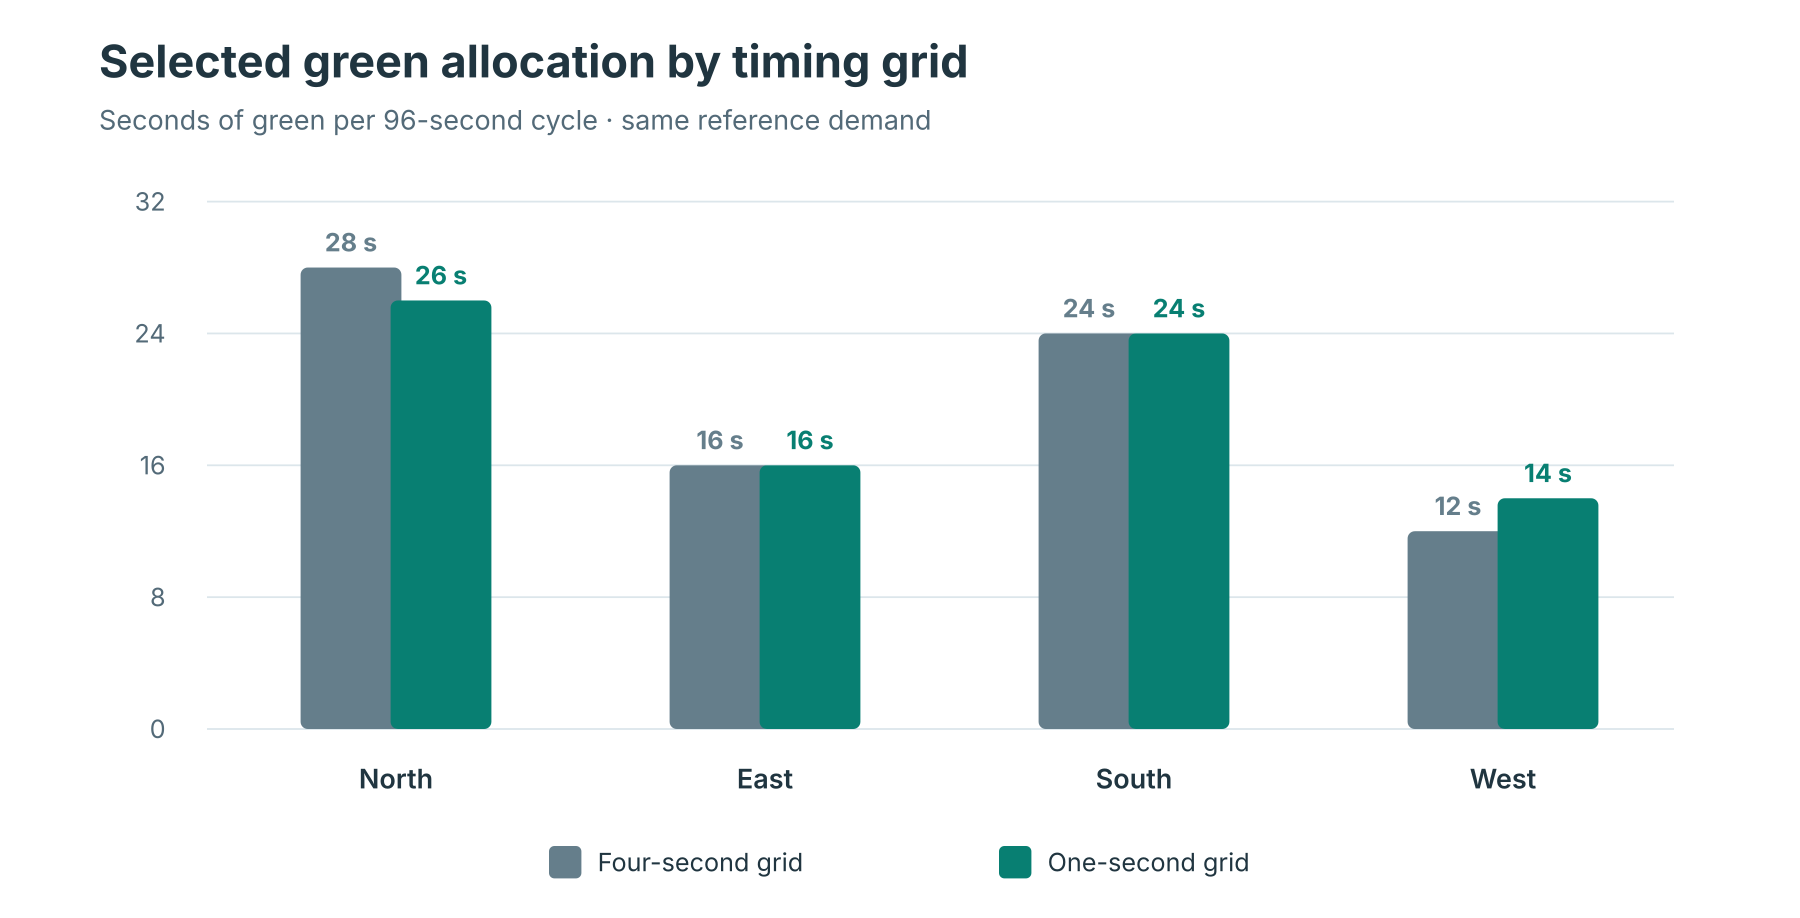
\includegraphics[width=\linewidth,height=0.55\textheight,keepaspectratio]{../assets/fig-grid-timing.png}
    \column{0.41\textwidth}
      \textbf{\large Selected green: 26 / 16 / 24 / 14 s}
      \begin{itemize}
        \setlength{\itemsep}{0.12cm}
        \item 19,369 feasible allocations; 128 training runs per candidate.
        \item Search runtime: \textbf{6.86 seconds}.
        \item On 5,000 matched fresh runs: \textbf{44.8 vehicle-seconds/run} saved (0.42\%).
        \item Paired 95\% interval: \textbf{34.8--54.8}.
      \end{itemize}
  \end{columns}
  \vspace{0.12cm}
  \small\color{Muted}This supports a small difference between the selected plans for this model; it does not establish a global optimum.
\end{frame}

% 7 — capacity stress result.
\begin{frame}{Heavy demand can exceed modeled capacity}
  \begin{columns}[T,onlytextwidth]
    \column{0.59\textwidth}
      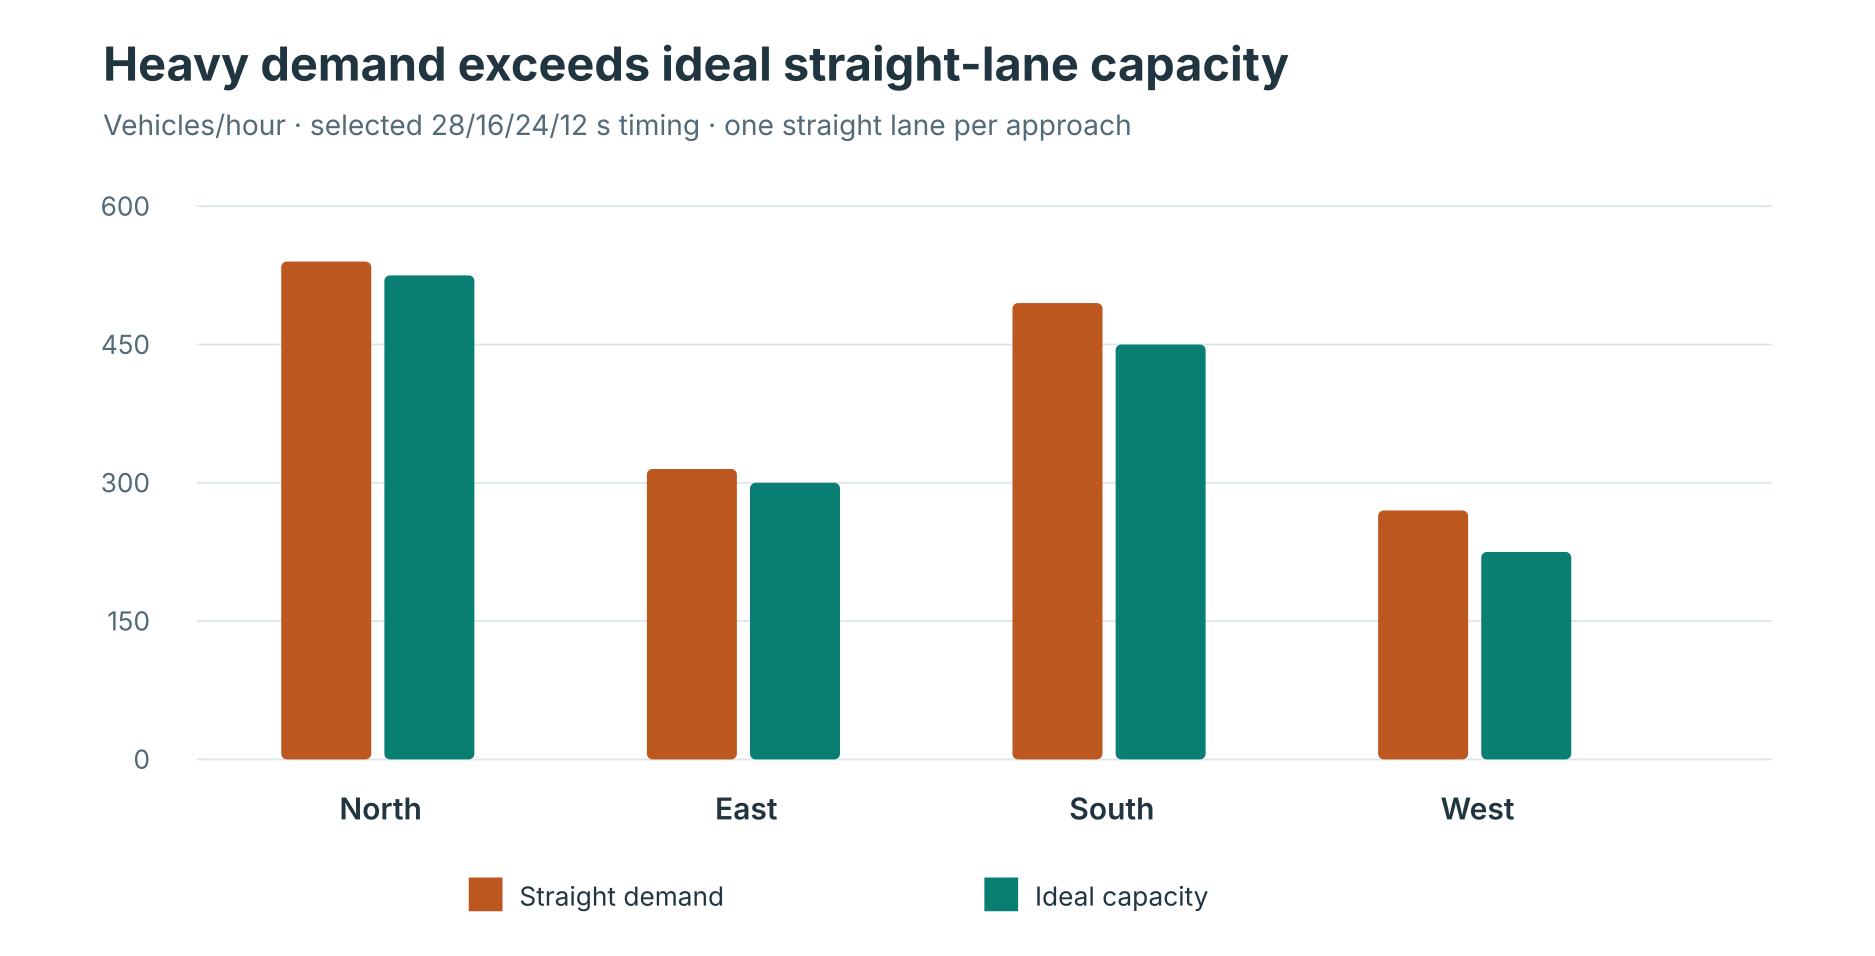
\includegraphics[width=\linewidth,height=0.58\textheight,keepaspectratio]{../assets/fig-capacity.png}
    \column{0.37\textwidth}
      \begin{itemize}
        \setlength{\itemsep}{0.28cm}
        \item Heavy-scenario arrival rate: \textbf{2,700 vehicles/hour}.
        \item Straight-stream demand requires \textbf{86.4 seconds} of green.
        \item Only \textbf{80 seconds} of green are available per cycle.
      \end{itemize}
  \end{columns}
  \vspace{0.18cm}
  \begin{block}{Residual queue}
    Mean backlog is 54.4 vehicles at 10 minutes and 110.1 vehicles at 32 minutes.
  \end{block}
\end{frame}

% 8 — horizon sensitivity and limits of interpretation.
\begin{frame}{Interpret the recommendation within its scope}
  \begin{columns}[T,onlytextwidth]
    \column{0.57\textwidth}
      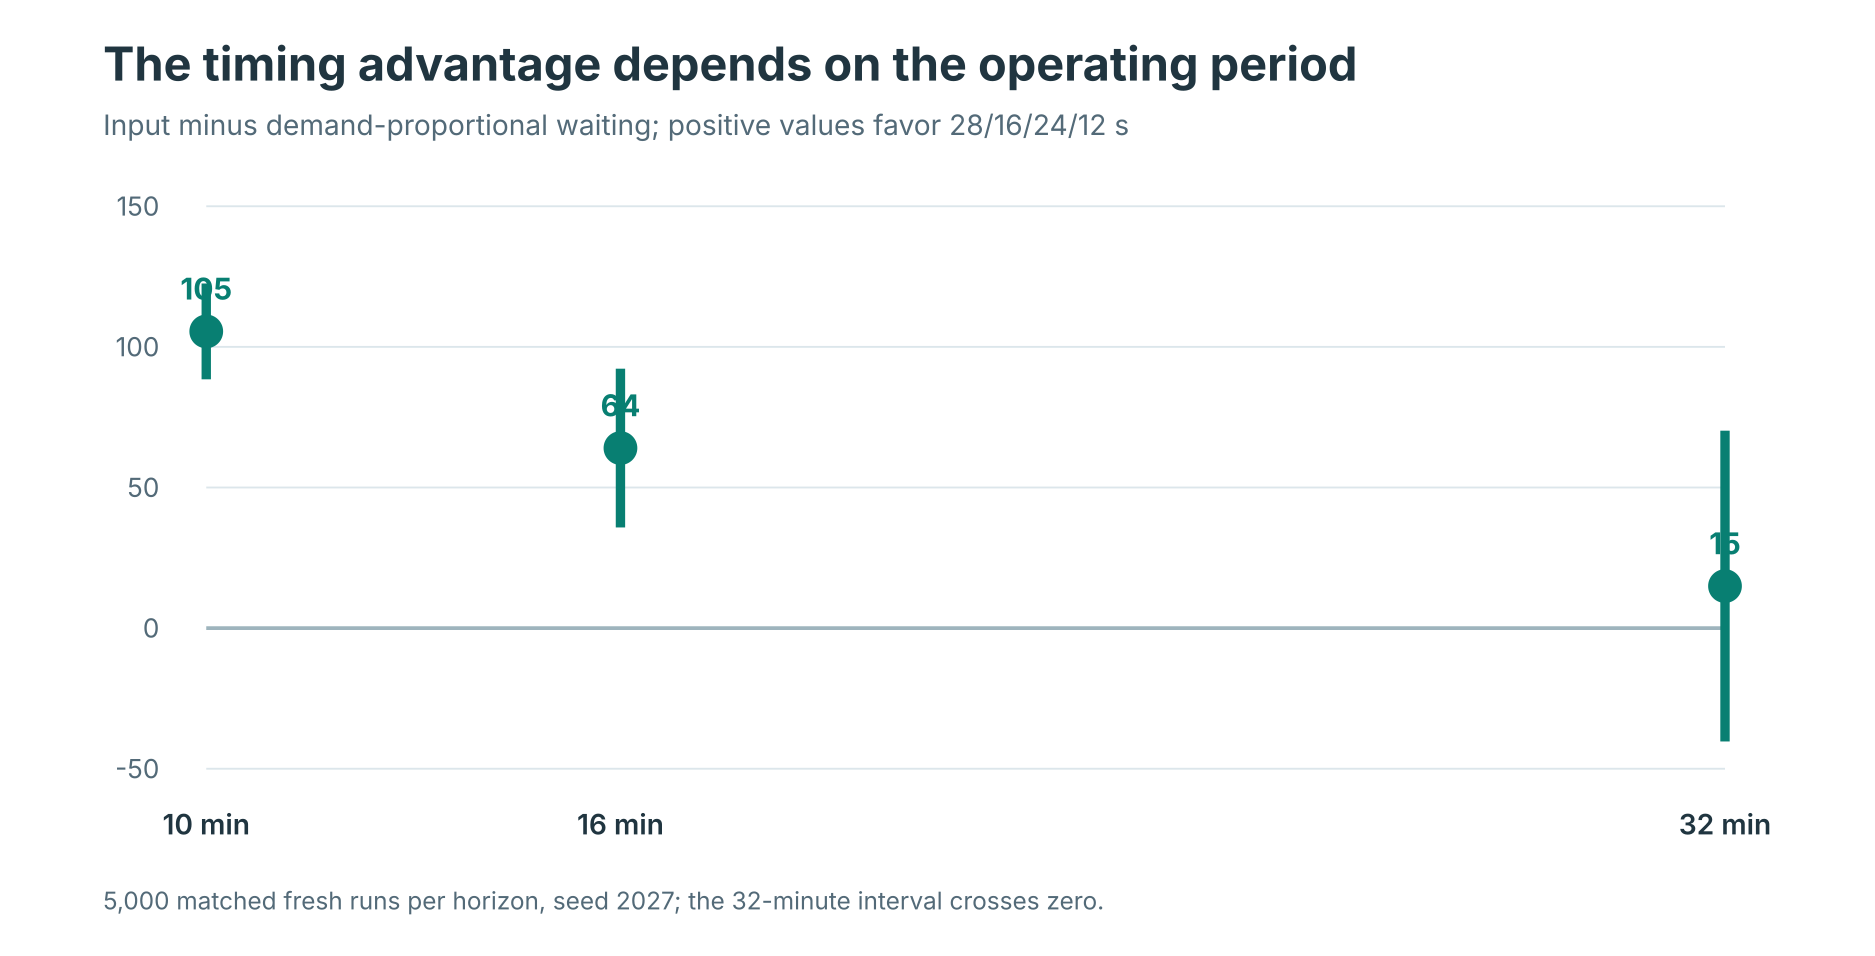
\includegraphics[width=\linewidth,height=0.58\textheight,keepaspectratio]{../assets/fig-horizon.png}
    \column{0.39\textwidth}
      \begin{block}{10-minute horizon}
        Saving: \textbf{105.5 vehicle-seconds/run}\\
        Paired 95\% interval: 88.5--122.5.
      \end{block}
      \begin{alertblock}{32-minute horizon}
        Saving: \textbf{15.0 vehicle-seconds/run}\\
        Paired 95\% interval: $-40.3$--70.2; no resolved difference.
      \end{alertblock}
  \end{columns}
  \vspace{0.18cm}
  \small\color{Muted}Field counts and calibration are needed before applying the timing outside this model.
\end{frame}

\end{document}
